\section{Auswertung}
\label{sec:Auswertung}

\subsection{Stabilitätsbedingung}
Gemäß Formel \ref{eqn:} wird die Stabilitätsbedingung für die beiden getroffenen Spiegelkonstatlationen im folgenden Untersucht. In Abbildung \ref{fig:stabi} sind die Spiegelparameter in Abhängikeit der Krümmungsradien aufgetragen. 
\begin{figure}
  \centering
  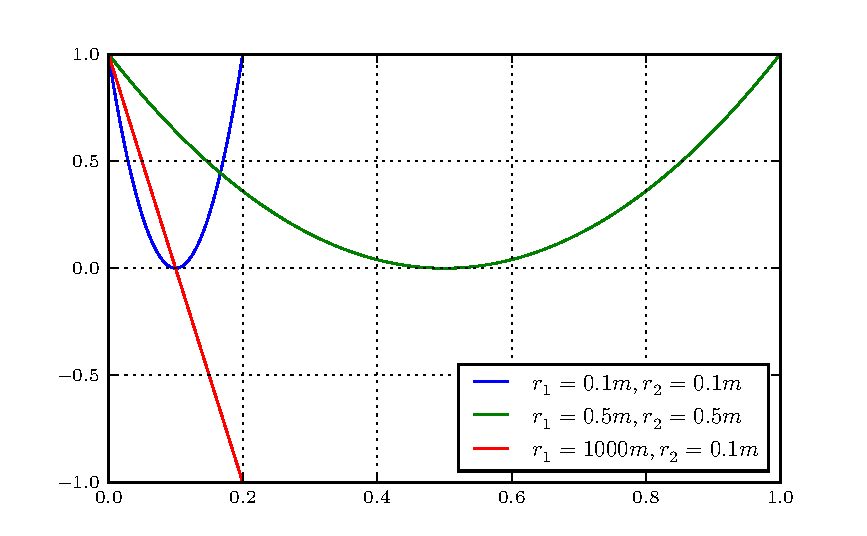
\includegraphics[height=6cm]{Stabilisationsparameter.pdf} 
  \caption{Stabilitätsbedingung des Resonators}
  \label{fig:stabi}
\end{figure}
Aus dem Diagramm lässt sich ablesen, dass bei Verwendung zweier Spiegel mit einem Krümmungsradius von 
\begin{equation}
  r_1 = 1400 \text{m}
  \label{eqn:rad1}
\end{equation}
die Maximal zu erwartenden Reichweite
\begin{equation}
  R_\text{1 max} = 2.8 \, \text{m}
  \label{eqn:rmax1}
\end{equation}
ist. Dies kann jedoch im Experiment nicht verifiziert werden, da die Schiene auf welche die Resonatorspiegel sitzen zu kurz ist. Bei der Verwedung von einem graden und einem Spiegel des Radiuses $r_1$ ergibt sich eine theoretische Reichweite von
\begin{equation}
  R_\text{2 max} = 1.4 \, \text{m} \ .
  \label{eqn:rmax2}
\end{equation}
Diese Reichweite wird verifiziert indem die Intensität der gemessenen Laserstrahlung von 100 \mu A bei einem Resonator abstand von 140 auf 2 \mu A abfällt. 

\subsection{TEM-Moden}

\subsubsection{TEM$_\text{00}$-Mode}
\begin{figure}
  \centering
  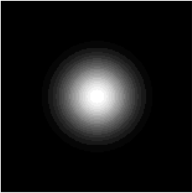
\includegraphics[height=6cm]{TEM00.pdf}
  \caption{<+caption text+>}
  \label{fig:<+label+>}
\end{figure}<++>
\subsubsection{TEM$_\text{01}$-Mode}
\begin{figure}
  \centering
  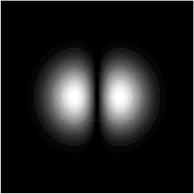
\includegraphics[height=6cm]{TEM10.pdf}
  \caption{<+caption text+>}
  \label{fig:<+label+>}
\end{figure}<++>

\subsection{Polarisation der Laserstrahlung}

\begin{figure}
  \centering
  \includegraphics[height=6cm]{Polar.pdf}
  \caption{<+caption text+>}
  \label{fig:<+label+>}
\end{figure}<++>
\subsection{Wellenlänge des Lasers}

